% !TeX program = xelatex
\documentclass[a4paper,10pt]{article}

% ============================================================================
% សន្លឹកកិច្ចការសិស្សបំពេញចន្លោះ ស-ខ្មៅ និងប្លង់ក្ដារខៀន/ចម្លើយគ្រូ (គ្មាន LCD / គ្មានកន្ត្រៃ)
% មេរៀនទី៤ (២)៖ ម៉ាសធៀបនឹងផ្ទៃក្រឡា — ត្រូវគ្នា ១០០% នឹង LS_Plan_MEAS42.tex
% ============================================================================
\usepackage[a4paper, left=1.0cm, right=1.0cm, top=0.75cm, bottom=1.00cm, footskip=0.52cm]{geometry}
\usepackage{amsmath}
\usepackage{unicode-math}
\usepackage{fontspec}
\usepackage{array, colortbl}
\usepackage[table]{xcolor}
\usepackage{enumitem}
\usepackage{pifont}
\usepackage{fancyhdr}
\usepackage{lastpage}
\usepackage{tikz}
\usepackage[most]{tcolorbox}
\usetikzlibrary{calc, arrows.meta, decorations.pathreplacing, positioning, babel}

\makeatletter
\let\@expl@@@mark@update@singlecol@structures@@\relax
\makeatother

\providecommand{\NGSFindFonts}{%
  \IfFileExists{C:/Windows/Fonts/cambria.ttc}{%
    \def\NGSSysPath{C:/Windows/Fonts/}%
    \def\NGSUserPath{C:/Users/KIT/AppData/Local/Microsoft/Windows/Fonts/}%
  }{%
    \IfFileExists{./fonts/KhmerOSsiemreap.ttf}{\def\NGSSysPath{./fonts/}\def\NGSUserPath{./fonts/}}{%
    \IfFileExists{../fonts/KhmerOSsiemreap.ttf}{\def\NGSSysPath{../fonts/}\def\NGSUserPath{../fonts/}}{%
    \IfFileExists{../../fonts/KhmerOSsiemreap.ttf}{\def\NGSSysPath{../../fonts/}\def\NGSUserPath{../../fonts/}}{%
    \IfFileExists{../../../fonts/KhmerOSsiemreap.ttf}{\def\NGSSysPath{../../../fonts/}\def\NGSUserPath{../../../fonts/}}{%
    \IfFileExists{../../../../fonts/KhmerOSsiemreap.ttf}{\def\NGSSysPath{../../../../fonts/}\def\NGSUserPath{../../../../fonts/}}{%
    \IfFileExists{../../../../../fonts/KhmerOSsiemreap.ttf}{\def\NGSSysPath{../../../../../fonts/}\def\NGSUserPath{../../../../../fonts/}}{%
    \IfFileExists{../../../../../../fonts/KhmerOSsiemreap.ttf}{\def\NGSSysPath{../../../../../../fonts/}\def\NGSUserPath{../../../../../../fonts/}}{%
      \def\NGSSysPath{../../../../../../../fonts/}\def\NGSUserPath{../../../../../../../fonts/}%
    }}}}}}}%
  }%
}
\NGSFindFonts

\setmathfont[Path={\NGSSysPath}, FontIndex=1, Scale=1.02]{cambria.ttc}
\defaultfontfeatures{Ligatures=TeX}

\setmainfont[
  Path={\NGSUserPath}, Extension=.ttf, Script=Khmer,
  BoldFont={KhmerOSsiemreap}, BoldFeatures={FakeBold=1.8},
  ItalicFont={KhmerOSsiemreap}, ItalicFeatures={FakeSlant=0.25},
  BoldItalicFont={KhmerOSsiemreap}, BoldItalicFeatures={FakeBold=1.8, FakeSlant=0.25}
]{KhmerOSsiemreap}

\newfontfamily\muol[Path={\NGSUserPath}, Extension=.ttf, Script=Khmer]{KhmerOSmuollight}
\newfontfamily\TimesEn[Path={\NGSSysPath}, Extension=.ttf, BoldFont={timesbd}, ItalicFont={timesi}, BoldItalicFont={timesbi}]{times}
\newfontfamily\CalibriFont[Path={\NGSSysPath}, Extension=.ttf]{calibri}

\XeTeXlinebreaklocale "km"
\XeTeXlinebreakskip = 0pt plus 1pt minus 0.1pt

\definecolor{panelgray}{gray}{0.94}
\definecolor{headgray}{gray}{0.85}

\pagestyle{fancy}
\fancyhf{}
\renewcommand{\headrulewidth}{0pt}
\fancyfoot[L]{\fontsize{7.4pt}{9.5pt}\selectfont អនុវិទ្យាល័យព្រះក្រសាំង \en{|} គ្រូ៖ ហុក ប៊ុនថែន \en{|} មេរៀនទី៤ (២) ម៉ាសធៀបនឹងផ្ទៃក្រឡា \en{|} ថ្ងៃអង្គារ ទី១ ខែធ្នូ ឆ្នាំ២០២៦}
\fancyfoot[R]{\fontsize{7.8pt}{10pt}\selectfont ទំព័រ \en{\thepage\ / \pageref{LastPage}}}

\setlength{\parindent}{0pt}
\setlength{\parskip}{0pt}
\setlength{\tabcolsep}{4pt}

\newcommand{\en}[1]{{\TimesEn #1}}
\newcommand{\enbf}[1]{{\TimesEn\bfseries #1}}
\newcommand{\unit}[1]{\,\text{\en{#1}}}
\newcommand{\riel}{\,\text{៛}}
\newcommand{\cnum}[1]{\mbox{\fontsize{10pt}{12pt}\selectfont\ding{\numexpr181+#1\relax}}}
\newcommand{\chkbox}{\tikz[baseline=-0.15ex]\draw[black, line width=0.85pt, fill=white] (0,0) rectangle (0.24cm,0.24cm);}
\newcommand{\ansbox}[1][1.75cm]{\,\tikz[baseline=-0.65ex]\draw[black, line width=0.65pt, fill=white] (0,0) rectangle (#1, 0.42cm);\,}
\newcommand{\dotline}[1][2.2cm]{\makebox[#1]{\dotfill}}

\newcommand{\pagebanner}[2]{%
  \begin{tcolorbox}[
    enhanced, sharp corners, colback=headgray, colframe=black,
    boxrule=1.05pt, boxsep=1pt, top=2.5pt, bottom=2.5pt, left=6pt, right=6pt,
    after skip=3.5pt
  ]
    {\muol\fontsize{9.0pt}{13.2pt}\selectfont #1}\hfill{\fontsize{8.0pt}{11.2pt}\selectfont\textbf{#2}}
  \end{tcolorbox}%
}

\newcommand{\secstrip}[2]{%
  \vspace{3pt}%
  \begin{tcolorbox}[
    enhanced, sharp corners, colback=panelgray, colframe=black,
    boxrule=0.8pt, boxsep=0.8pt, top=2pt, bottom=2pt, left=5pt, right=5pt,
    after skip=3pt
  ]
    {\muol\fontsize{8.5pt}{12.2pt}\selectfont #1}\hfill{\fontsize{7.8pt}{10.8pt}\selectfont\textit{#2}}
  \end{tcolorbox}%
}

\newcolumntype{L}[1]{>{\raggedright\arraybackslash}p{#1}}
\newcolumntype{C}[1]{>{\centering\arraybackslash}p{#1}}

\begin{document}
\fontsize{9.5pt}{14.5pt}\selectfont

% ============================================================================
% ទំព័រទី ១៖ សន្លឹកកិច្ចការសិស្ស (ផ្នែកមុខ៖ E1 -> E2 -> E3)
% ============================================================================
\pagebanner{សន្លឹកកិច្ចការសិស្ស \enbf{(}៤\enbf{.}២ ម៉ាសធៀបនឹងផ្ទៃក្រឡា\enbf{)} \enbf{--} ផ្នែកមុខ}{ថ្នាក់ទី៨ \en{|} សៀវភៅគោល ទំ.៤៤--៤៥}

\begin{tcolorbox}[
  enhanced, sharp corners, colback=white, colframe=black,
  boxrule=0.8pt, boxsep=1.5pt, top=3.5pt, bottom=3.5pt, left=5pt, right=5pt,
  after skip=4pt
]
  \fontsize{9.0pt}{13.0pt}\selectfont
  \textbf{ឈ្មោះសិស្ស៖} \dotline[4.3cm] \quad
  \textbf{សមាជិកក្រុម៖} \dotline[4.3cm] \quad
  \textbf{ថ្នាក់ទី៖} ៨\dotline[0.9cm] \quad
  \textbf{ក្រុមទី៖} \dotline[1.0cm]
\end{tcolorbox}

% --- E1 Engage ---
\secstrip{ផ្នែកទី ១ \enbf{(E1 - Engage)} ៖ បេសកកម្មស្លាកកញ្ចប់ក្រដាសរ៉ាម $80\unit{g/m}^2$}{រយៈពេល ៣ នាទី (គូស \ding{51} ក្នុង \chkbox)}

\begin{tcolorbox}[
  enhanced, sharp corners, colback=white, colframe=black,
  boxrule=0.8pt, boxsep=2pt, top=3.5pt, bottom=3.5pt, left=6pt, right=6pt
]
  នៅលើកញ្ចប់ក្រដាសរ៉ាមខ្នាត $\unit{A4}$ ($210\unit{mm}\times 297\unit{mm}$) មានសរសេរស្លាកសម្គាល់កម្រាស់ថា $80\unit{g/m}^2$ ៖\\[2pt]
  $\bullet$ \textbf{តើមតិមួយណាបកស្រាយអត្ថន័យ $80\unit{g/m}^2$ បានត្រឹមត្រូវ?} \quad
  \chkbox\ \textbf{សិស្ស ក៖} $\unit{A4}$ ១ សន្លឹកធ្ងន់ $80\unit{g}$ \qquad
  \chkbox\ \textbf{សិស្ស ខ៖} ផ្ទៃ $1\unit{m}^2$ ធ្ងន់ $80\unit{g}$ (ឯ $\unit{A4}$ ១ សន្លឹក $\approx 5\unit{g}$)\\[2pt]
  $\bullet$ \textbf{ហេតុផលខ្លី៖} តើសន្លឹកកិច្ចការ $\unit{A4}$ មួយសន្លឹកនេះធំជាង ឬតូចជាងផ្ទៃការេ $1\unit{m}\times 1\unit{m}$? \dotline[5.4cm] ។
\end{tcolorbox}

\vfill

% --- E2 Explore ---
\secstrip{ផ្នែកទី ២ \enbf{(E2 - Explore)} ៖ លំហាត់គំរូទី ១ — ម៉ាសក្រដាសរ៉ាម ១ ដុំ $500$ សន្លឹក (ទំ.៤៤--៤៥)}{រយៈពេល ១១ នាទី}

\textbf{សកម្មភាព ១ (\en{E2-A} — ៦ នាទី)៖ គណនាម៉ាសក្រដាសរ៉ាម ១ ដុំ ($500$ សន្លឹក, ខ្នាត $210\unit{mm}\times 297\unit{mm}, d = 80\unit{g/m}^2$)}

\begin{tcolorbox}[
  enhanced, sharp corners, colback=white, colframe=black,
  boxrule=0.8pt, boxsep=2pt, top=3.5pt, bottom=3.5pt, left=6pt, right=6pt
]
  $\bullet$ \textbf{កម្រាស់ក្រដាស (ទំ.៤៤)៖} សៀវភៅក្រាស់ $50\unit{g/m}^2$, សៀវភៅស្ដើង/រ៉ាម $80\unit{g/m}^2$, ក្របសៀវភៅ $200\unit{g/m}^2$ ។\\[3pt]
  $\bullet$ \textbf{ជំហាន \cnum{1} — ផ្ទៃក្រដាស ១ សន្លឹក ($S$)៖} $S = 210\times 10^{-3}\unit{m} \times 297\times 10^{-3}\unit{m} =$ \ansbox[2.6cm] $\unit{m}^2$\\[3pt]
  $\bullet$ \textbf{ជំហាន \cnum{2} — បំប្លែងម៉ាសធៀបនឹងផ្ទៃក្រឡា ($d$)៖} $d = 80\unit{g/m}^2 = 80\times$ \dotline[1.4cm] $\unit{kg/m}^2$\\[3pt]
  $\bullet$ \textbf{ជំហាន \cnum{3} — ម៉ាសក្រដាស ១ សន្លឹក ($m_1$)៖} $m_1 = S\times d = 62\,370\times 10^{-6}\times 80\times 10^{-3} =$ \dotline[2.5cm] $\unit{kg}$\\[3pt]
  $\bullet$ \textbf{ជំហាន \cnum{4} — ម៉ាសក្រដាសរ៉ាម ១ ដុំ ($500$ សន្លឹក)៖} $m = 500\times m_1 =$ \dotline[2.4cm] $\unit{kg} \approx$ \ansbox[1.8cm] $\unit{kg}$
\end{tcolorbox}

\vspace{3pt}
\textbf{សកម្មភាព ២ (\en{E2-B} — ៥ នាទី)៖ ពិនិត្យអន្ទាក់ភ្លេចបំប្លែង $\unit{g} \to \unit{kg}$ និងអន្ទាក់យក $80\unit{g}\times 500$}

\begin{tcolorbox}[
  enhanced, sharp corners, colback=white, colframe=black,
  boxrule=0.8pt, boxsep=2pt, top=3.5pt, bottom=3.5pt, left=6pt, right=6pt
]
  $\bullet$ \textbf{អន្ទាក់ទី ១៖} បើភ្លេចបំប្លែង $80\unit{g/m}^2$ ជា $80\times 10^{-3}\unit{kg/m}^2$ នោះចម្លើយនឹងធំជាងការពិត \dotline[1.6cm] ដង ($2\,494.8\unit{kg}$)!\\[2.5pt]
  $\bullet$ \textbf{អន្ទាក់ទី ២៖} បើច្រឡំយក $80\unit{g}\times 500$ សន្លឹក នោះបាន $40\,000\unit{g} =$ \dotline[1.4cm] $\unit{kg}$ (ខុសការពិតជិត $16$ ដង!) ។
\end{tcolorbox}

\vfill

% --- E3 Explain ---
\secstrip{ផ្នែកទី ៣ \enbf{(E3 - Explain)} ៖ រូបមន្តម៉ាសធៀបនឹងផ្ទៃក្រឡា និងធនាគារហេតុផល \enbf{B\&W}}{រយៈពេល ៦ នាទី}

\begin{tcolorbox}[
  enhanced, sharp corners, colback=white, colframe=black,
  boxrule=0.85pt, boxsep=2pt, top=3.5pt, bottom=3.5pt, left=6pt, right=6pt
]
  ១) \textbf{បំប្លែងខ្នាត៖} $1\unit{g/m}^2 =$ \dotline[1.2cm] $\unit{kg/m}^2$ \qquad
  ២) \textbf{ម៉ាស ១ សន្លឹក៖} $m_1 = S\times \dotline[0.9cm]$ \qquad
  ៣) \textbf{ម៉ាស $N$ សន្លឹក៖} $m = N\times S\times d$\\[3pt]
  ៤) \textbf{ពេលកាត់ខាតចំនៀរ $r\%$៖} $S_{\text{ខាត}} = S_{\text{សុទ្ធ}}\times \dfrac{r}{100} \implies S_{\text{សរុប}} = S_{\text{សុទ្ធ}} + \dotline[1.4cm] \implies m = S_{\text{សរុប}}\times d$\\[4pt]
  \tikz\draw[black, dashed, line width=0.5pt] (0,0) -- (18.4cm,0);\\[3pt]
  \fontsize{8.8pt}{12.8pt}\selectfont
  \textbf{ធនាគារហេតុផល (\en{Warrant Bank})៖} \quad
  \cnum{1} \textbf{ផ្ទៃ ១ សន្លឹក៖} បំប្លែង $\unit{mm}\to 10^{-3}\unit{m}$ មុនគុណ $S = a\times b$ \quad
  \cnum{2} \textbf{ខ្នាត $d$៖} $1\unit{g/m}^2 = 10^{-3}\unit{kg/m}^2$\\
  \cnum{3} \textbf{ក្រដាស ១ រ៉ាម៖} $S_{500} = 500\times S_1$ \quad
  \cnum{4} \textbf{បូកចំនៀរខាត $r\%$៖} $S_{\text{សរុប}} = S_{\text{សុទ្ធ}} + S_{\text{ខាត}}$ រួចគណនា $m = S_{\text{សរុប}}\times d$
\end{tcolorbox}

% ============================================================================
% ទំព័រទី ២៖ សន្លឹកកិច្ចការសិស្ស (ផ្នែកខាងខ្នង៖ E4 -> E5 -> កិច្ចការផ្ទះ)
% ============================================================================
\clearpage
\pagebanner{សន្លឹកកិច្ចការសិស្ស \enbf{(}៤\enbf{.}២ ម៉ាសធៀបនឹងផ្ទៃក្រឡា\enbf{)} \enbf{--} ផ្នែកខាងខ្នង}{ថ្នាក់ទី៨ \en{|} សៀវភៅគោល ទំ.៤៥--៤៦, ៥០}

% --- E4 Elaborate ---
\secstrip{ផ្នែកទី ៤ \enbf{(E4 - Elaborate)} ៖ លំហាត់គំរូទី ២ — កាត់ក្រដាសខ្នាតធំខាតចំនៀរ $4\%$ (ទំ.៤៥--៤៦)}{រយៈពេល ១០ នាទី}

\begin{tcolorbox}[
  enhanced, sharp corners, colback=white, colframe=black,
  boxrule=0.8pt, boxsep=2pt, top=3.5pt, bottom=3.5pt, left=6pt, right=6pt
]
  \textbf{លំហាត់គំរូទី ២ (ទំ.៤៥--៤៦)៖} គេទិញក្រដាសខ្នាតធំដែលមានម៉ាសធៀបនឹងផ្ទៃក្រឡា $d = 70\unit{g/m}^2$ មកកាត់ជាក្រដាសរ៉ាមខ្នាត $210\unit{mm}\times 297\unit{mm}$ ដោយត្រូវខាតបង់ចំនៀរក្រដាសអស់ $4\%$ ។ ដើម្បីបានក្រដាសរ៉ាម ១ ដុំ ($500$ សន្លឹក) តើត្រូវប្រើអស់ក្រដាសប៉ុន្មាន $\unit{kg}$?\\[3pt]
  $\bullet$ \textbf{ជំហាន \cnum{1} និង \cnum{3}៖} ផ្ទៃ ១ សន្លឹក $S_1 = 62\,370\times 10^{-6}\unit{m}^2 \implies$ ផ្ទៃ ១ ដុំ $S_{500} = 500\times S_1 =$ \dotline[2.4cm] $\unit{m}^2$\\[3pt]
  $\bullet$ \textbf{ជំហាន \cnum{4} — ផ្ទៃត្រូវខាត $4\%$៖} $S_{\text{ខាត}} = S_{500}\times \dfrac{4}{100} =$ \dotline[2.3cm] $\unit{m}^2 \implies S_{\text{សរុប}} =$ \dotline[2.4cm] $\unit{m}^2$\\[3pt]
  $\bullet$ \textbf{ជំហាន \cnum{2} — ម៉ាសក្រដាសសរុប៖} $m = 70\times 10^{-3}\times S_{\text{សរុប}} =$ \dotline[2.4cm] $\unit{kg} \approx$ \ansbox[1.8cm] $\unit{kg}$\\[2pt]
  \fontsize{8.7pt}{12.5pt}\selectfont
  \textbf{ឆ្លុះបញ្ចាំង (\en{EIA Looking-Back})៖} គេត្រូវ\textbf{បូក}ផ្ទៃខាត $4\%$ បន្ថែម ព្រោះចំនៀរក្រដាសត្រូវ \dotline[3.6cm] នៅពេលកាត់ ។
\end{tcolorbox}

\vfill

% --- E5 Evaluate ---
\secstrip{ផ្នែកទី ៥ \enbf{(E5 - Evaluate)} ៖ លំហាត់ប្រតិបត្តិ (ទំ.៤៦) សំណួរវិនិច្ឆ័យ \enbf{A--D} និងសំបុត្រចេញ}{រយៈពេល ១០ នាទី}

\begin{tcolorbox}[
  enhanced, sharp corners, colback=white, colframe=black,
  boxrule=0.8pt, boxsep=2pt, top=3.5pt, bottom=3.5pt, left=6pt, right=6pt
]
  \textbf{១) ប្រតិបត្តិ (ទំ.៤៦)៖} សិប្បកម្មខ្នាតតូចមួយទិញក្រដាសខ្នាតធំមាន $d = 80\unit{g/m}^2$ មកកាត់ជាក្រដាសរ៉ាមខ្នាត $210\unit{mm}\times 297\unit{mm}$ ដោយខាតចំនៀរអស់ $4\%$ ។ ដើម្បីបានក្រដាស $95\,340$ រ៉ាម តើគេត្រូវប្រើអស់ក្រដាសប៉ុន្មាន $\unit{kg}$?\\[3pt]
  $\bullet$ ផ្ទៃក្រដាសសរុបសម្រាប់ ១ រ៉ាម (រួមទាំងខាត $4\%$)៖ $S_{\text{រ៉ាម}} = 31.185\times 1.04 =$ \dotline[2.2cm] $\unit{m}^2$\\[3pt]
  $\bullet$ ម៉ាសក្រដាសក្នុង ១ រ៉ាម (\cnum{2})៖ $m_{\text{រ៉ាម}} = 80\times 10^{-3}\times S_{\text{រ៉ាម}} =$ \dotline[2.3cm] $\unit{kg}$\\[3pt]
  $\bullet$ ម៉ាសក្រដាសសរុបសម្រាប់ $95\,340$ រ៉ាម៖ $m = 95\,340\times m_{\text{រ៉ាម}} \approx$ \ansbox[2.8cm] $\unit{kg}$\\[3pt]
  \textbf{២) បិទបេសកកម្ម \en{E1}៖} មតិសិស្ស \dotline[0.9cm] ត្រឹមត្រូវ ព្រោះក្រដាស $\unit{A4}$ ១ សន្លឹកមានម៉ាស $m_1 \approx$ \dotline[1.4cm] $\unit{g}$ ប៉ុណ្ណោះ ។
\end{tcolorbox}

\vspace{3.5pt}

\begin{tcolorbox}[
  enhanced, sharp corners, colback=white, colframe=black,
  boxrule=0.8pt, boxsep=2pt, top=3.5pt, bottom=3.5pt, left=6pt, right=6pt
]
  \textbf{៣) សំណួរវិនិច្ឆ័យ \en{A--D} (ក្របសៀវភៅ $200\unit{g/m}^2$ ផ្ទៃ ១ សន្លឹក $= 0.5\unit{m}^2$ ចំនួន $100$ សន្លឹក តើមានម៉ាសប៉ុន្មាន $\unit{kg}$? — លើកម្រាមដៃ ១--៤)៖}\\[2.5pt]
  \textbf{\en{A.}} $10\,000\unit{kg}$ \qquad
  \textbf{\en{B.}} $10\unit{kg}$ \qquad
  \textbf{\en{C.}} $20\unit{kg}$ \qquad
  \textbf{\en{D.}} $0.1\unit{kg}$\\[3.5pt]
  \tikz\draw[black, dashed, line width=0.5pt] (0,0) -- (18.4cm,0);\\[3pt]
  \textbf{៤) សំបុត្រចេញ ៦០ វិនាទី៖} ប័ណ្ណរឹងទំហំ $10\unit{cm}\times 20\unit{cm}$ ($S_1 =$ \dotline[1.5cm] $\unit{m}^2$) កម្រាស់ $250\unit{g/m}^2$ ចំនួន $1\,000$ សន្លឹក៖
  ផ្ទៃសរុប $=$ \dotline[1.5cm] $\unit{m}^2$, \quad ម៉ាសសរុប $m =$ \dotline[1.6cm] $\unit{kg}$ ។
\end{tcolorbox}

\vfill

% --- Homework ---
\begin{tcolorbox}[
  enhanced, sharp corners, colback=panelgray, colframe=black,
  boxrule=0.95pt, boxsep=2pt, top=3.5pt, bottom=3.5pt, left=6pt, right=6pt
]
  {\muol\fontsize{9.0pt}{13.0pt}\selectfont កិច្ចការផ្ទះ \enbf{(}សៀវភៅគោល ទំ.៥០ លេខ ៥ ក និង ខ\enbf{)}}\\[2.5pt]
  \fontsize{8.8pt}{13.0pt}\selectfont
  $\bullet$ \textbf{\#5 (ទំ.៥០)៖} សៀវភៅសរសេរមួយក្បាលមាន $100$ ទំព័រ ($= 50$ សន្លឹកសាច់ក្នុង និងក្របមុខ-ក្រោយ $2$ សន្លឹក) មានខ្នាត $148\unit{mm}\times 210\unit{mm}$ ។ គេប្រើក្រដាស $70\unit{g/m}^2$ ធ្វើសាច់ក្នុង និងក្រដាស $150\unit{g/m}^2$ ធ្វើក្របសៀវភៅ ។ \textbf{ក.} គេផលិត $10\,000$ ក្បាល តើត្រូវការក្រដាសសរុបប៉ុន្មាន $\unit{kg}$ បើខាតចំនៀរអស់ $4\%$? \quad \textbf{ខ.} បើក្រដាស $1\unit{kg}$ ថ្លៃ $4\,800\riel$ រកប្រាក់ដើមថ្លៃក្រដាសនៃសៀវភៅ ១ ក្បាល ។ \textbf{អានមុន៖} ៣. ម៉ាសធៀបនឹងមាឌ (ទំ.៤៦--៤៨) ។
\end{tcolorbox}

% ============================================================================
% ទំព័រទី ៣៖ ទំព័រគ្រូបង្រៀន (គំរូប្លង់ក្ដារខៀន ៣ ផ្នែក + ចម្លើយផ្ទៀងផ្ទាត់រហ័ស)
% ============================================================================
\clearpage
\pagebanner{ទំព័រគ្រូបង្រៀន ៖ ប្លង់ក្ដារខៀន \enbf{(}គ្មាន \enbf{LCD)} និងចម្លើយផ្ទៀងផ្ទាត់រហ័ស}{៤.២ ម៉ាសធៀបនឹងផ្ទៃក្រឡា (\en{MEAS42})}

\secstrip{១. គំរូប្លង់បែងចែកក្ដារខៀន ៣ ផ្នែក សម្រាប់ថ្នាក់រៀនគ្មាន \enbf{LCD}}{សម្រាប់គ្រូប្រើដីស/ហ្វឺត}

\begin{center}
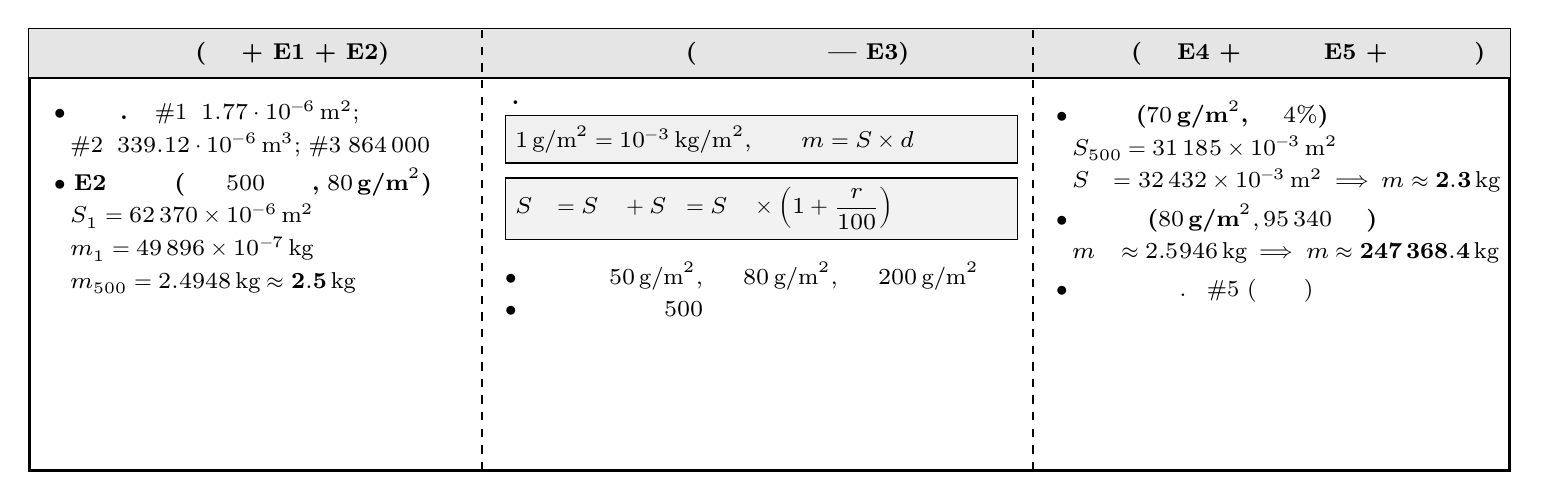
\begin{tikzpicture}[x=1cm, y=1cm, every node/.style={font=\fontsize{8.3pt}{11.8pt}\selectfont, text=black}]
  \draw[black, line width=1.1pt] (0,0) rectangle (18.8,5.60);
  \fill[gray!20] (0,4.98) rectangle (18.8,5.60);
  \draw[black, line width=0.7pt] (0,4.98) -- (18.8,4.98);
  \draw[black, dashed, line width=0.7pt] (5.75,0) -- (5.75,5.60);
  \draw[black, dashed, line width=0.7pt] (12.75,0) -- (12.75,5.60);

  \node at (2.875,5.29) {\textbf{ផ្នែកឆ្វេង (កំណែ + \en{E1} + \en{E2})}};
  \node at (9.25,5.29) {\textbf{ផ្នែកកណ្ដាល (ខ្លឹមសារគោលរក្សាទុក — \en{E3})}};
  \node at (15.775,5.29) {\textbf{ផ្នែកស្ដាំ (គំរូ \en{E4} + ប្រតិបត្តិ \en{E5} + កិច្ចការផ្ទះ)}};

  % Left
  \node[anchor=north west, text width=5.35cm] at (0.20,4.82) {%
    $\bullet$ \textbf{កំណែ ទំ.៥០៖} \#1ក $1.77\cdot 10^{-6}\unit{m}^2$;\\
    \hspace*{0.2cm}\#2ក $339.12\cdot 10^{-6}\unit{m}^3$; \#3 $864\,000\riel$\\[2pt]
    $\bullet$ \textbf{\en{E2} គំរូទី ១ (១ ដុំ $500$ សន្លឹក, $80\unit{g/m}^2$)៖}\\
    \hspace*{0.2cm}$S_1 = 62\,370\times 10^{-6}\unit{m}^2$\\
    \hspace*{0.2cm}$m_1 = 49\,896\times 10^{-7}\unit{kg}$\\
    \hspace*{0.2cm}$m_{500} = 2.4948\unit{kg} \approx \mathbf{2.5\unit{kg}}$
  };

  % Center
  \node[anchor=north west, text width=6.65cm] at (5.92,4.82) {%
    {\muol\fontsize{8.5pt}{12pt}\selectfont ២\enbf{.} ម៉ាសធៀបនឹងផ្ទៃក្រឡា}\\[3pt]
    \tikz\node[draw=black, fill=gray!12, inner sep=3.5pt, text width=6.25cm]{%
      $1\unit{g/m}^2 = 10^{-3}\unit{kg/m}^2, \qquad m = S\times d$
    };\\[4pt]
    \tikz\node[draw=black, fill=gray!10, inner sep=3.5pt, text width=6.25cm]{%
      $S_{\text{សរុប}} = S_{\text{សុទ្ធ}} + S_{\text{ខាត}} = S_{\text{សុទ្ធ}}\times\left(1 + \dfrac{r}{100}\right)$
    };\\[4pt]
    $\bullet$ ក្រដាសក្រាស់ $50\unit{g/m}^2$, រ៉ាម $80\unit{g/m}^2$, ក្រប $200\unit{g/m}^2$\\
    $\bullet$ ក្រដាសរ៉ាម ១ ដុំ មាន $500$ សន្លឹក
  };

  % Right
  \node[anchor=north west, text width=5.8cm] at (12.92,4.82) {%
    $\bullet$ \textbf{គំរូទី ២ ($70\unit{g/m}^2$, ខាត $4\%$)៖}\\
    \hspace*{0.2cm}$S_{500} = 31\,185\times 10^{-3}\unit{m}^2$\\
    \hspace*{0.2cm}$S_{\text{សរុប}} = 32\,432\times 10^{-3}\unit{m}^2 \implies m \approx \mathbf{2.3\unit{kg}}$\\[2pt]
    $\bullet$ \textbf{ប្រតិបត្តិ ($80\unit{g/m}^2, 95\,340$ រ៉ាម)៖}\\
    \hspace*{0.2cm}$m_{\text{រ៉ាម}} \approx 2.5946\unit{kg} \implies m \approx \mathbf{247\,368.4\unit{kg}}$\\[2pt]
    $\bullet$ \textbf{កិច្ចការផ្ទះ៖} ទំ.៥០ \#5 (ក និង ខ)
  };
\end{tikzpicture}
\end{center}

\vspace{4pt}
\secstrip{២. ចម្លើយផ្ទៀងផ្ទាត់រហ័សសម្រាប់សន្លឹកកិច្ចការសិស្ស \enbf{(}ទំព័រ ១ និង ទំព័រ ២\enbf{)}}{\en{Answer Key}}

\begin{tcolorbox}[
  enhanced, sharp corners, colback=white, colframe=black,
  boxrule=0.8pt, boxsep=2pt, top=4pt, bottom=4pt, left=6pt, right=6pt
]
  \fontsize{9.0pt}{13.6pt}\selectfont
  $\bullet$ \textbf{ផ្នែក \en{E1}៖} \textbf{មតិសិស្ស ខ} ត្រឹមត្រូវ (ក្រដាស $\unit{A4}$ ១ សន្លឹកតូចជាង $1\unit{m}^2$ ជិត $16$ ដង និងធ្ងន់ $\approx 5\unit{g}$) ។\\[2pt]
  $\bullet$ \textbf{ផ្នែក \en{E2}៖} \textbf{សកម្មភាព ១៖} $S = 62\,370\times 10^{-6}\unit{m}^2, \ d = 80\times 10^{-3}\unit{kg/m}^2, \ m_1 = 49\,896\times 10^{-7}\unit{kg}, \ m = 2.4948\unit{kg} \approx 2.5\unit{kg}$ ។ \textbf{សកម្មភាព ២៖} ខុស $1\,000$ ដង; $40\unit{kg}$ ។\\[2pt]
  $\bullet$ \textbf{ផ្នែក \en{E4}៖} $S_{500} = 31\,185\times 10^{-3}\unit{m}^2, \ S_{\text{ខាត}} = 1\,247.4\times 10^{-3} \approx 1\,247\times 10^{-3}\unit{m}^2, \ S_{\text{សរុប}} = 32\,432\times 10^{-3}\unit{m}^2, \ m = 2.27024\unit{kg} \approx 2.3\unit{kg}$ ។\\[2pt]
  $\bullet$ \textbf{ផ្នែក \en{E5}៖} \textbf{១) ប្រតិបត្តិ៖} $S_{\text{រ៉ាម}} = 32.4324\unit{m}^2, \ m_{\text{រ៉ាម}} = 2.594592\unit{kg} \implies m \approx 247\,368.4\unit{kg}$ (បើតាម $32.432\unit{m}^2$ បាន $247\,365.4\unit{kg}$) ។ \textbf{២) បិទ \en{E1}៖} សិស្ស ខ ($\approx 5\unit{g}$) ។ \textbf{៣) វិនិច្ឆ័យ \en{A--D}៖} \textbf{ជម្រើស \en{B}} ($10\unit{kg}$) ។ \textbf{៤) សំបុត្រចេញ៖} $S_1 = 0.02\unit{m}^2, \ S_{\text{សរុប}} = 20\unit{m}^2, \ m = 5\unit{kg}$ ។
\end{tcolorbox}

\vspace{4pt}
\secstrip{៣. ចម្លើយលម្អិតនៃកិច្ចការផ្ទះ \enbf{(}សម្រាប់ផ្ទៀងនៅដើមម៉ោងបន្ទាប់ ៤\enbf{.}៣\enbf{)}}{សៀវភៅគោល ទំ.៥០}

\begin{tcolorbox}[
  enhanced, sharp corners, colback=white, colframe=black,
  boxrule=0.8pt, boxsep=2pt, top=4pt, bottom=4pt, left=6pt, right=6pt
]
  \fontsize{8.8pt}{13.2pt}\selectfont
  $\bullet$ \textbf{\#5 (ទំ.៥០ — សៀវភៅ $100$ ទំព័រ, ខ្នាត $148\unit{mm}\times 210\unit{mm}$, សាច់ក្នុង $70\unit{g/m}^2$, ក្រប $150\unit{g/m}^2$, $10\,000$ ក្បាល, ខាតចំនៀរ $4\%$)៖}\\[2pt]
  \hspace*{0.3cm}-- ផ្ទៃ ១ សន្លឹក ($148\unit{mm}\times 210\unit{mm}$)៖ $S_1 = 0.148\times 0.210 = 0.03108\unit{m}^2$ ។ ក្នុង ១ ក្បាលមានសាច់ក្នុង $50$ សន្លឹក ($= 100$ ទំព័រ) និងក្របមុខ-ក្រោយ $2$ សន្លឹក ៖\\[2pt]
  \hspace*{0.3cm}-- ម៉ាសសុទ្ធ ១ ក្បាល៖ $m_{\text{សាច់}} = 50\times 0.03108\times 0.070 = 0.10878\unit{kg}$ និង $m_{\text{ក្រប}} = 2\times 0.03108\times 0.150 = 0.009324\unit{kg} \implies m_{\text{សុទ្ធ}} = 0.118104\unit{kg}$ ។\\[2pt]
  \hspace*{0.3cm}-- \textbf{(ក)} បូកខាតចំនៀរ $4\%$ សម្រាប់ $10\,000$ ក្បាល៖ $m_{\text{សរុប}} = 10\,000\times 0.118104\times 1.04 = \mathbf{1\,228.28\unit{kg}}$; \quad \textbf{(ខ)} ថ្លៃក្រដាស ១ ក្បាល $= 0.122828\times 4\,800 \approx \mathbf{590\riel}$ ។
\end{tcolorbox}

\end{document}
